\documentclass[12pt,a4paper, hidelinks]{article}
\usepackage[utf8]{inputenc}
\usepackage{amsmath}
\usepackage{amsfonts}
\usepackage{amssymb}
\usepackage{amsthm}
\usepackage{graphicx}
\usepackage{hyperref}
\usepackage{geometry}
\geometry{a4paper, margin=1in}
\usepackage{fancyhdr}
\usepackage{indentfirst} % Add this line to enable first paragraph indentation
\usepackage{times} % Use Times New Roman font
\usepackage{setspace}
\usepackage{graphicx}
\usepackage{float}
\usepackage{listings}

\setstretch{1.15} % Adjust the stretch factor as needed

\pagestyle{fancy}
\fancyhf{}  % Clear header and footer fields
\rfoot{\thepage}  % Place page number at the right bottom corner
\renewcommand{\headrulewidth}{0pt}  % Remove the header line


\begin{document}

\section*{SKaMP. Tests}
\addcontentsline{toc}{section}{Introduction}
\vspace{\baselineskip} % Add an empty line after the section title

The goal of this report is to provide information on the performed testing of data acquisition, data pre-processing, batch processing and streaming processing.

GitHub repository: \href{https://github.com/salveendutt/Big-Data-Analytics}{https://github.com/salveendutt/Big-Data-Analytics}.

\section{Test Scenarios}

\begin{table}[h!]
\centering
\begin{tabular}{|p{3cm}|p{4cm}|p{3cm}|p{5cm}|}
\hline
\textbf{Test objective} & \textbf{Steps} & \textbf{Expected Result} & \textbf{Actual Result} \\
\hline
Verify data incoming from stream API & 1. Start the server using start\_containers.bat; 2. Navigate to http://localhost:5000 & Incoming data is available on /data/0 & Passed. The screenshot is provided in Figure \ref{fig:streaming-api} \\
\hline
Verify correct setup of the stream and data preprocessing functions & Run 'pytest' from the root folder & Data stream is configured as expected; Incoming data is not null; Returned status code - 200. Preprocessing utils return transformed data as expected & Passed. The screenshot is provided in Figure \ref{fig:unittests} \\
\hline
Verify the correct setup of Nifi - HDFS/Kafka flow & Run the containers - follow steps in README.md & Data flows from streamin API to Kafka topics and Hive tables & Passed. The screenshot is provided in Figure \ref{fig:kafka1}, \ref{fig:kafka2}, \ref{fig:kafka3}, \ref{fig:hive1} \\
\hline
Verify the correct setup of batch processing & Run the containers - follow steps in README.md & Views are available in the Cassandra tables & Passed. The screenshot is provided in Figure \ref{fig:cassandra-batch-1}, \ref{fig:cassandra-batch-2}, \ref{fig:cassandra-batch-3} \\
\hline
Verify the correct setup of streaming processing & Run the containers - follow steps in README.md & Views are available in the Cassandra tables & Passed. The screenshot is provided in Figure \ref{fig:cassandra-strean} \\
\hline
Verify that Superset correctly connects to Cassandra through TrinoDB and displays data in dashboards & Run the necessary containers (start\_containers) in 'scripts' folder and observe the charts in Superset &
Data is visible in Superset charts &
PASSED. Screenshots are visible in Figure x and x\\
\hline

\end{tabular}
\caption{Test scenarios}
\end{table}

\begin{table}[h!]
  \centering
  \begin{tabular}{|p{3cm}|p{2cm}|p{4cm}|p{5cm}|}
  \hline
  \textbf{Test objective} & \textbf{Steps} & \textbf{Expected Result} & \textbf{Actual Result} \\
  \hline
  Verify correct data pre-processing of dataset 1 & Run 'pytest' from the root folder & Feature 'type' is correctly transformed into numeric value (5 cases); Feature 'isMerchant' is correctly prepared (2 cases) & PASSED. The screenshot is provided in Figure \ref{fig:unittests} \\
  \hline
  Verify correct data pre-processing of dataset 2 & Run 'pytest' from the root folder & Numeric boolean values are transformed to int from float (4 cases) & PASSED. The screenshot is provided in Figure \ref{fig:unittests} \\
  \hline
  Verify correct data pre-processing of dataset 3 & Run 'pytest' from the root folder & Feature 'entry\_mode' is correctly transformed into numeric value (4 cases); Unnecessary features are omitted. & PASSED. The screenshot is provided in Figure \ref{fig:unittests} \\
  \hline
  Verify correct data pre-processing of dataset 4 & Run 'pytest' from the root folder & Features 'Amount', 'Class' are renamed to 'amount' and 'isFraud'; Extra features are removed & PASSED. The screenshot is provided in Figure \ref{fig:unittests} \\
  \hline
  \end{tabular}
  \caption{Data pre-processing tests}
  \end{table}

\begin{figure}[h!]
  \centering
  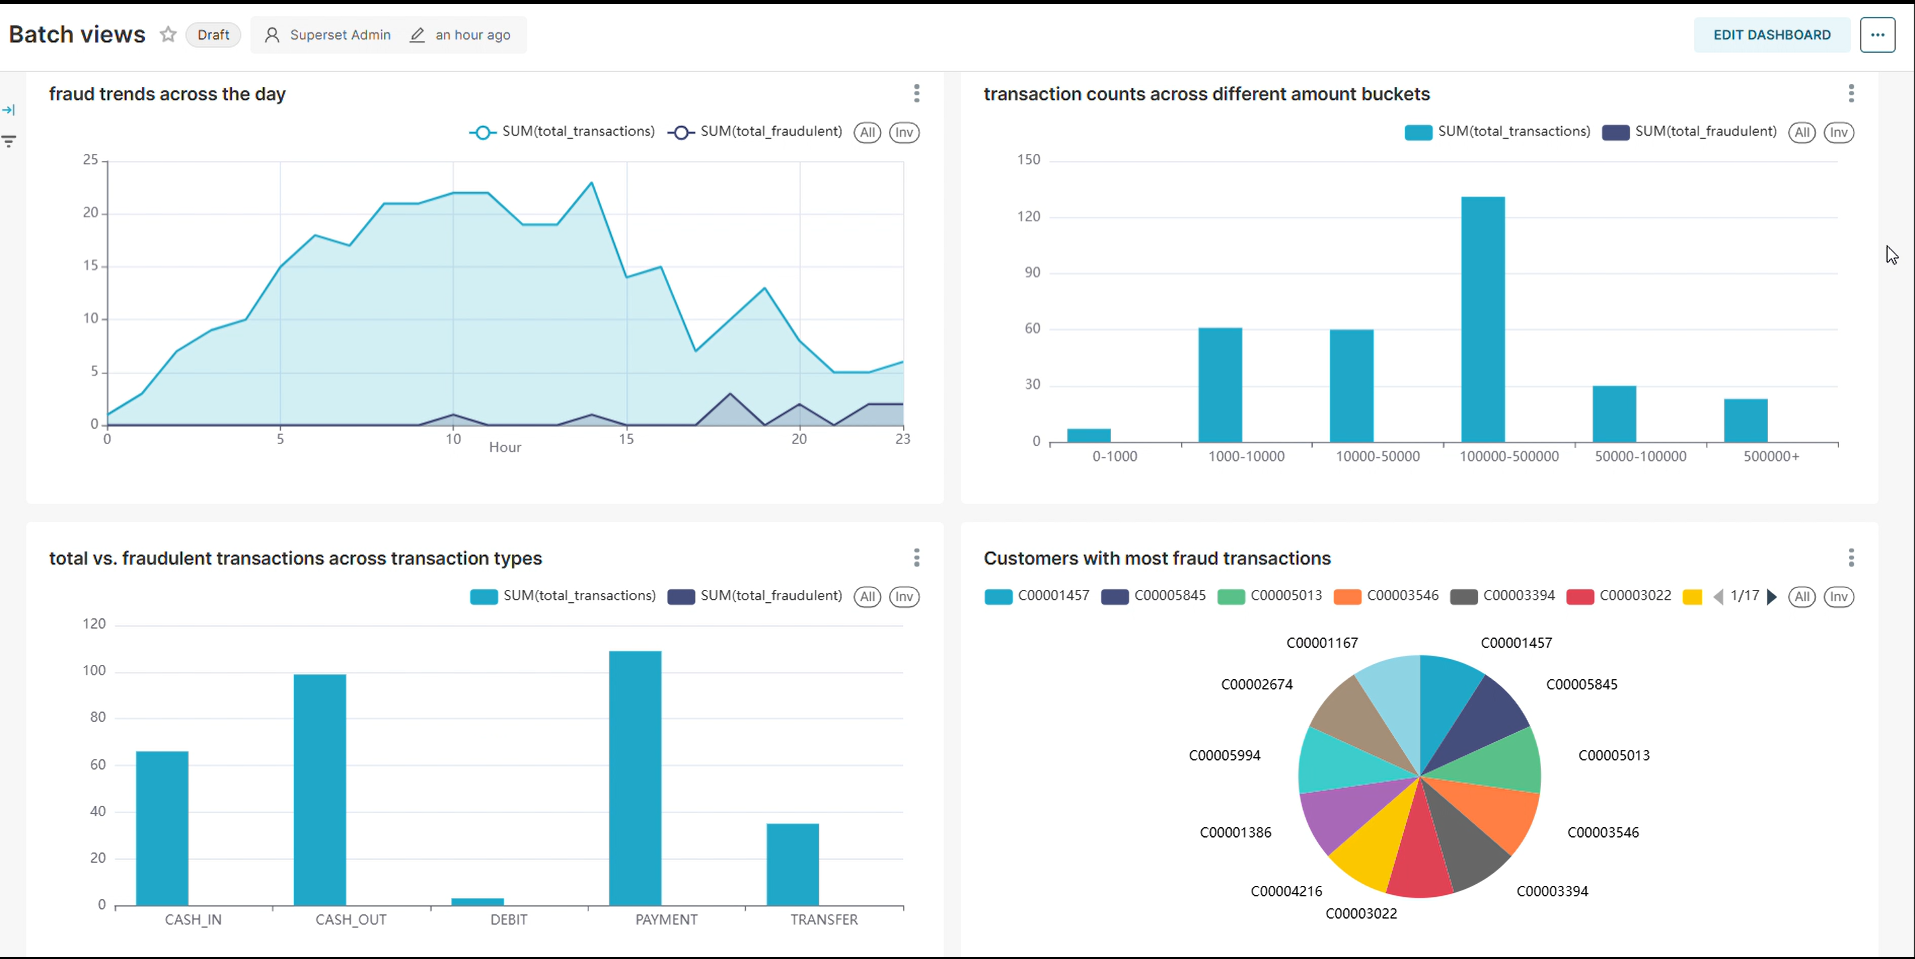
\includegraphics[width=0.8\textwidth]{images/superset-1.png}
  \caption{Batch Dashboard}
  \label{fig:batch-dashboard}
\end{figure}


\begin{figure}[h!]
  \centering
  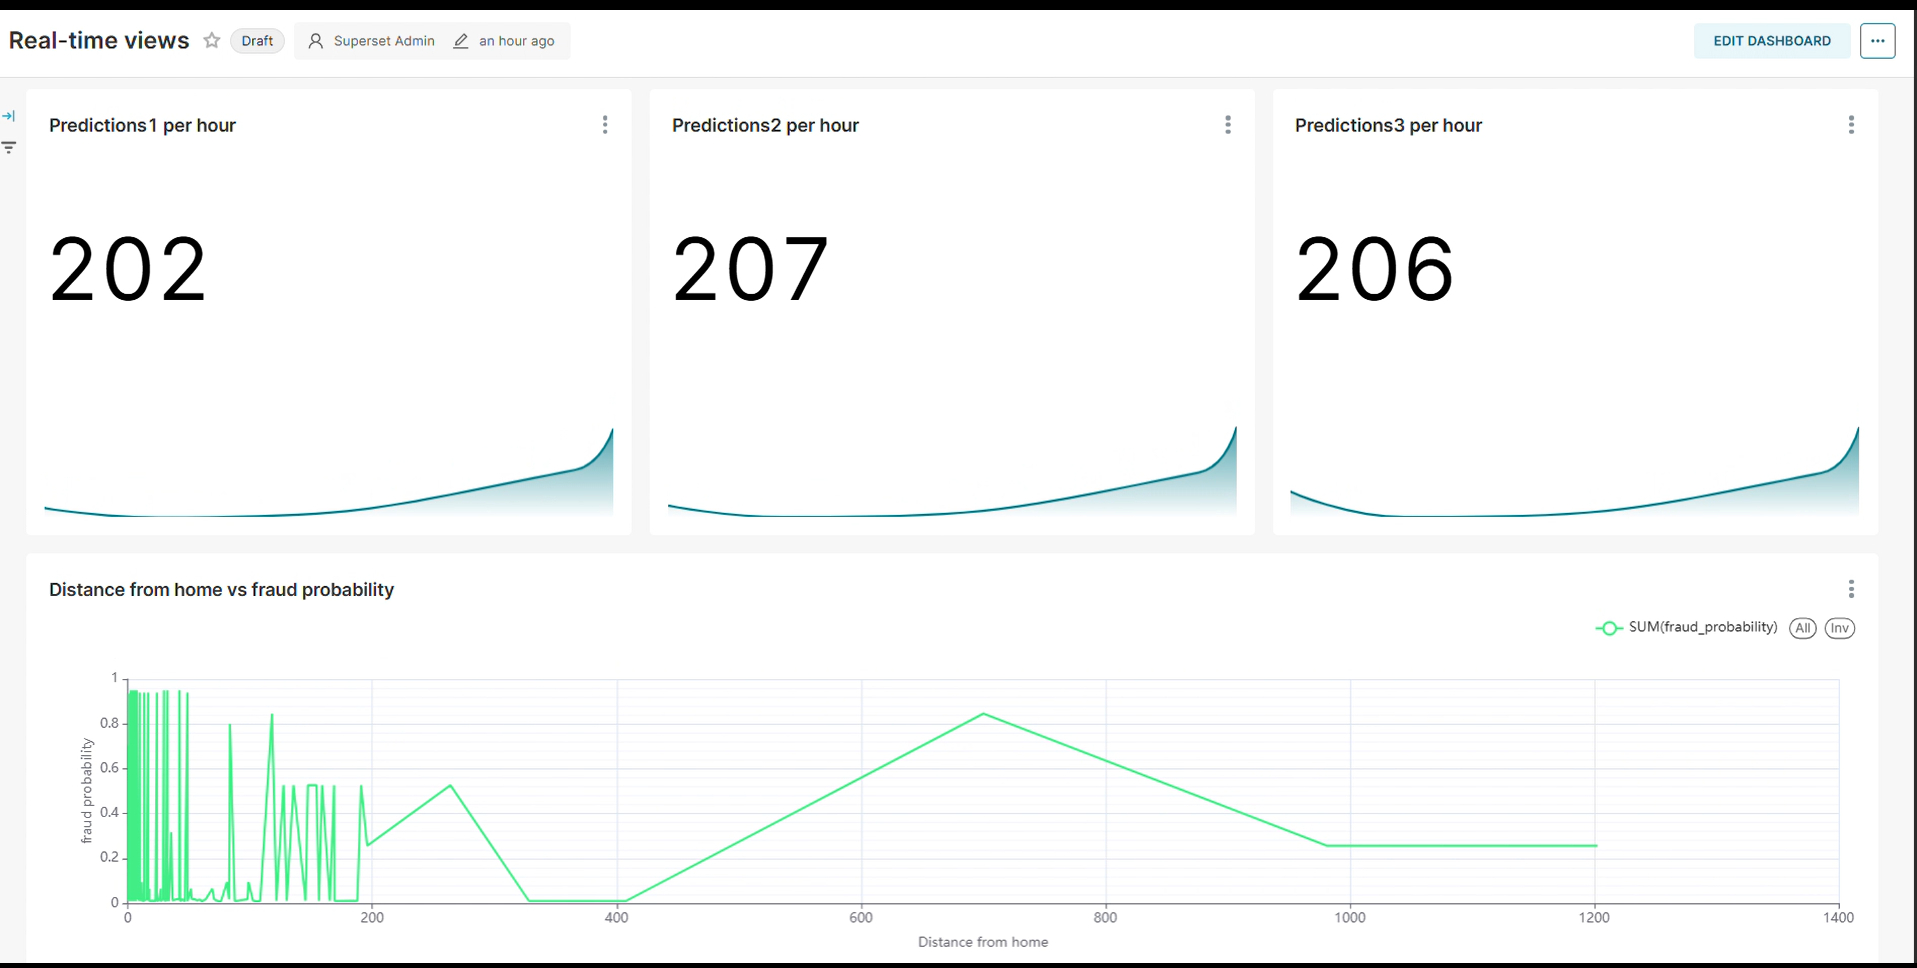
\includegraphics[width=0.8\textwidth]{images/superset-2.png}
  \caption{Speed Dashboard}
  \label{fig:speed-dashboard}
\end{figure}

\begin{figure}[h!]
  \centering
  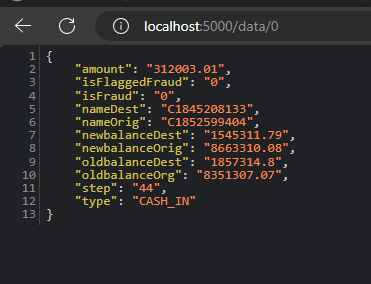
\includegraphics[width=0.8\textwidth]{images/test-stream-M2.png}
  \caption{Data incoming via the stream}
  \label{fig:streaming-api}
\end{figure}


\begin{figure}[h!]
  \centering
  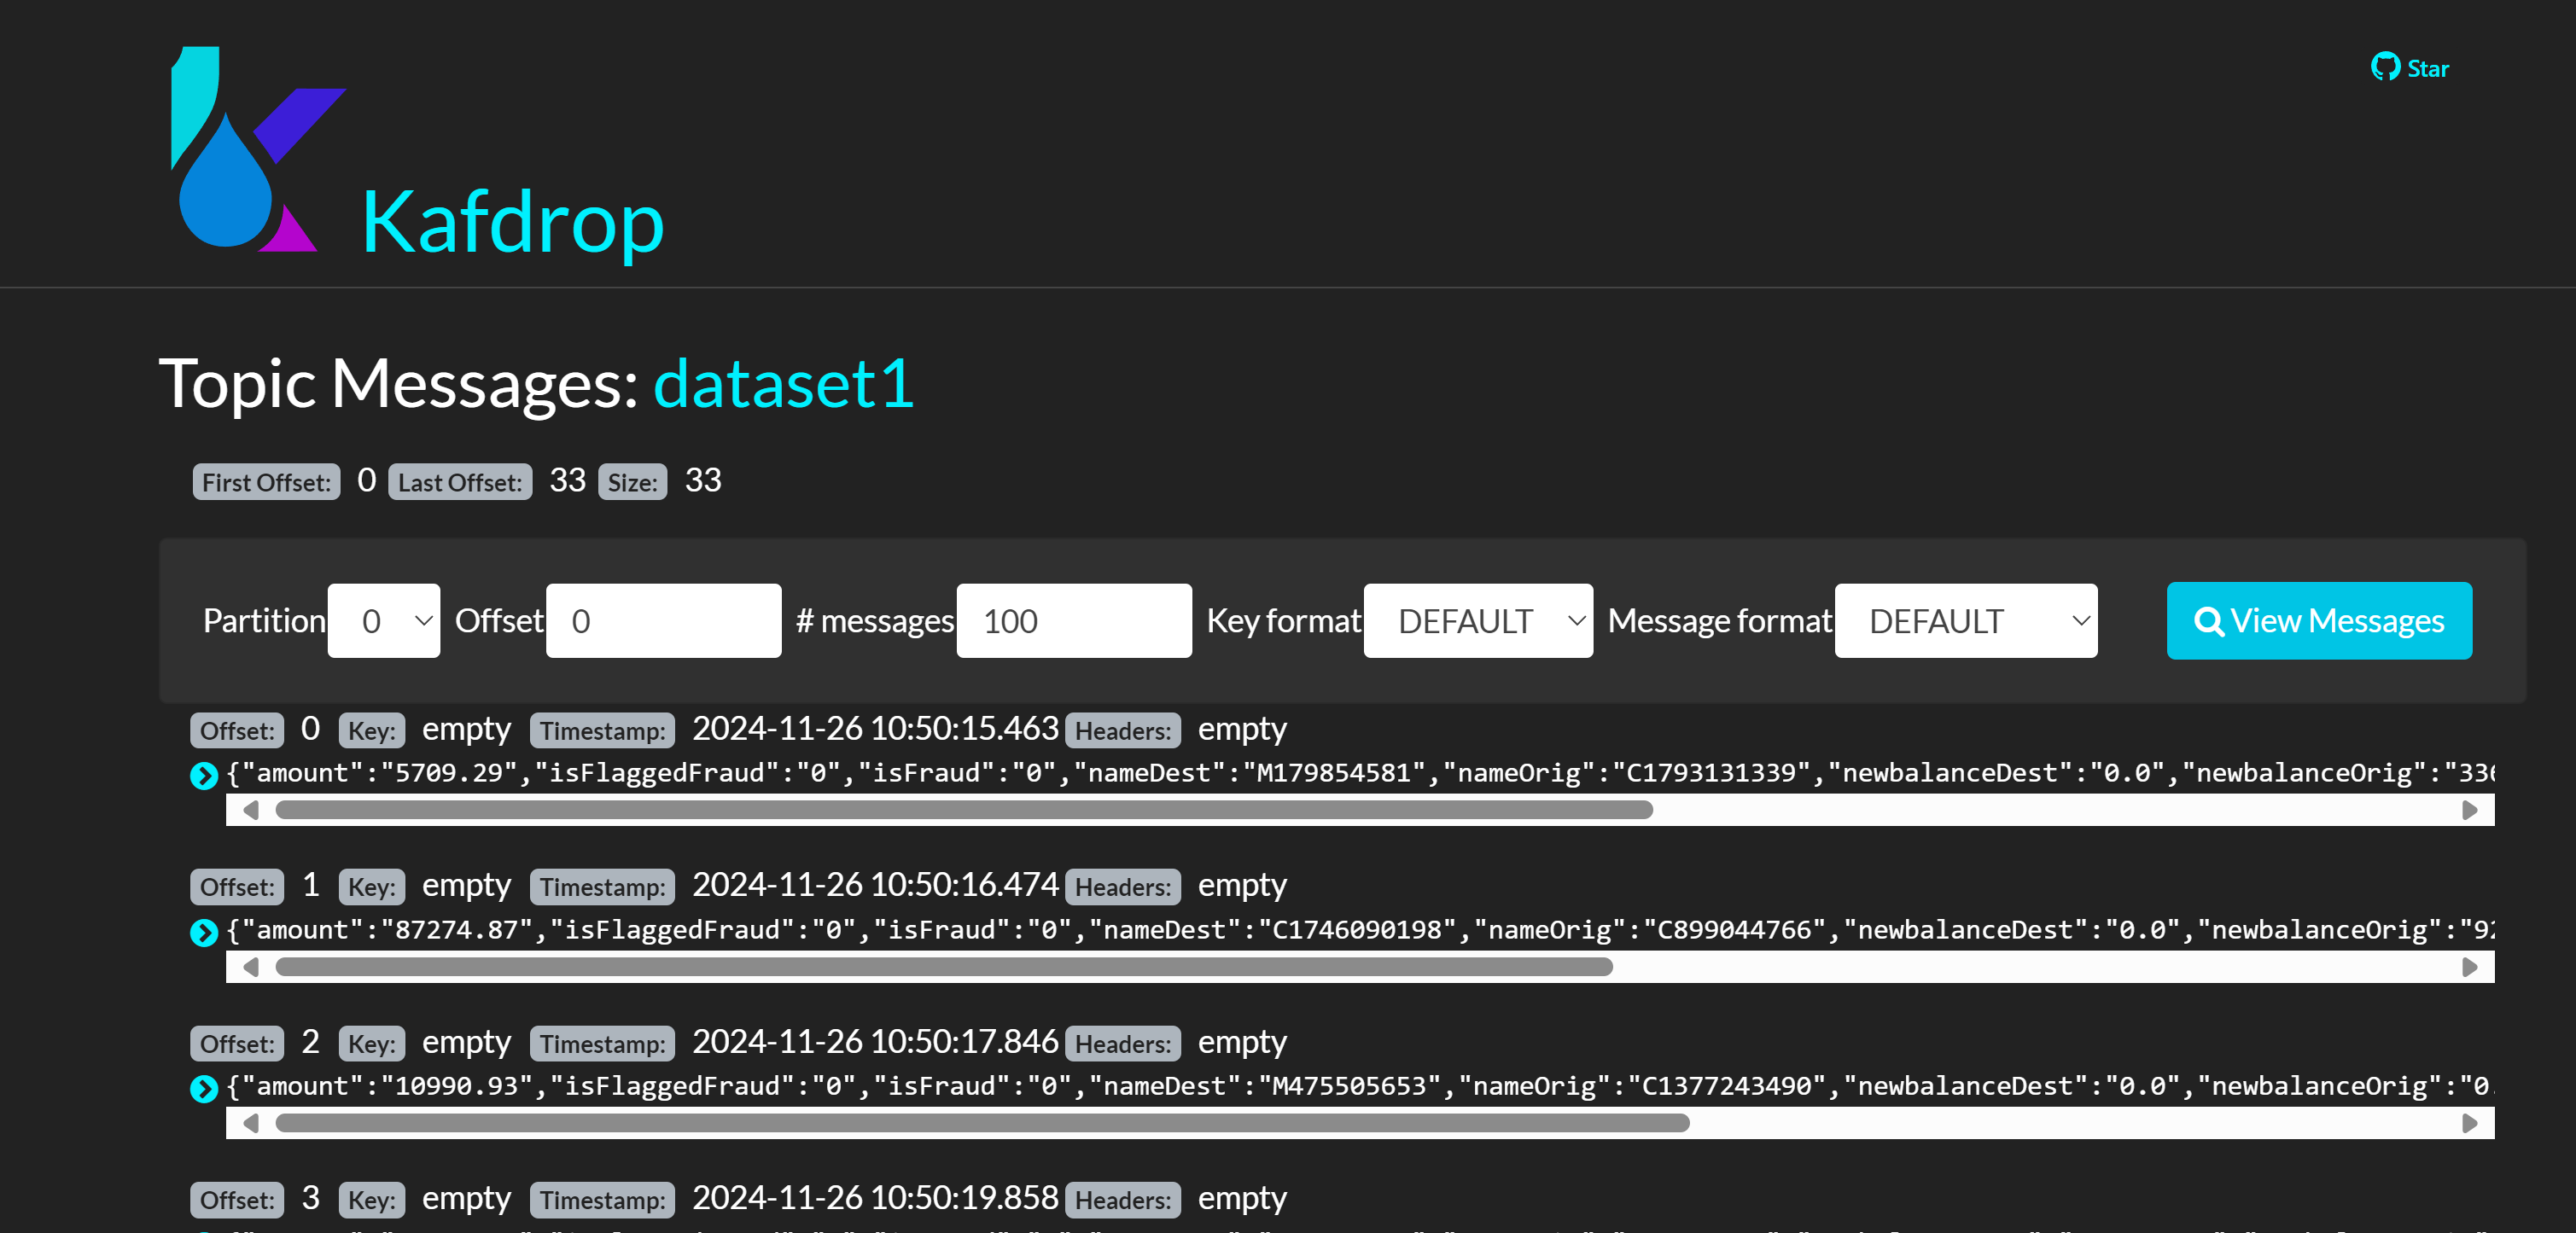
\includegraphics[width=0.95\textwidth]{images/m2-kafka-1.png}
  \caption{Kafka Dataset1}
  \label{fig:kafka1}
\end{figure}

\begin{figure}[h!]
  \centering
  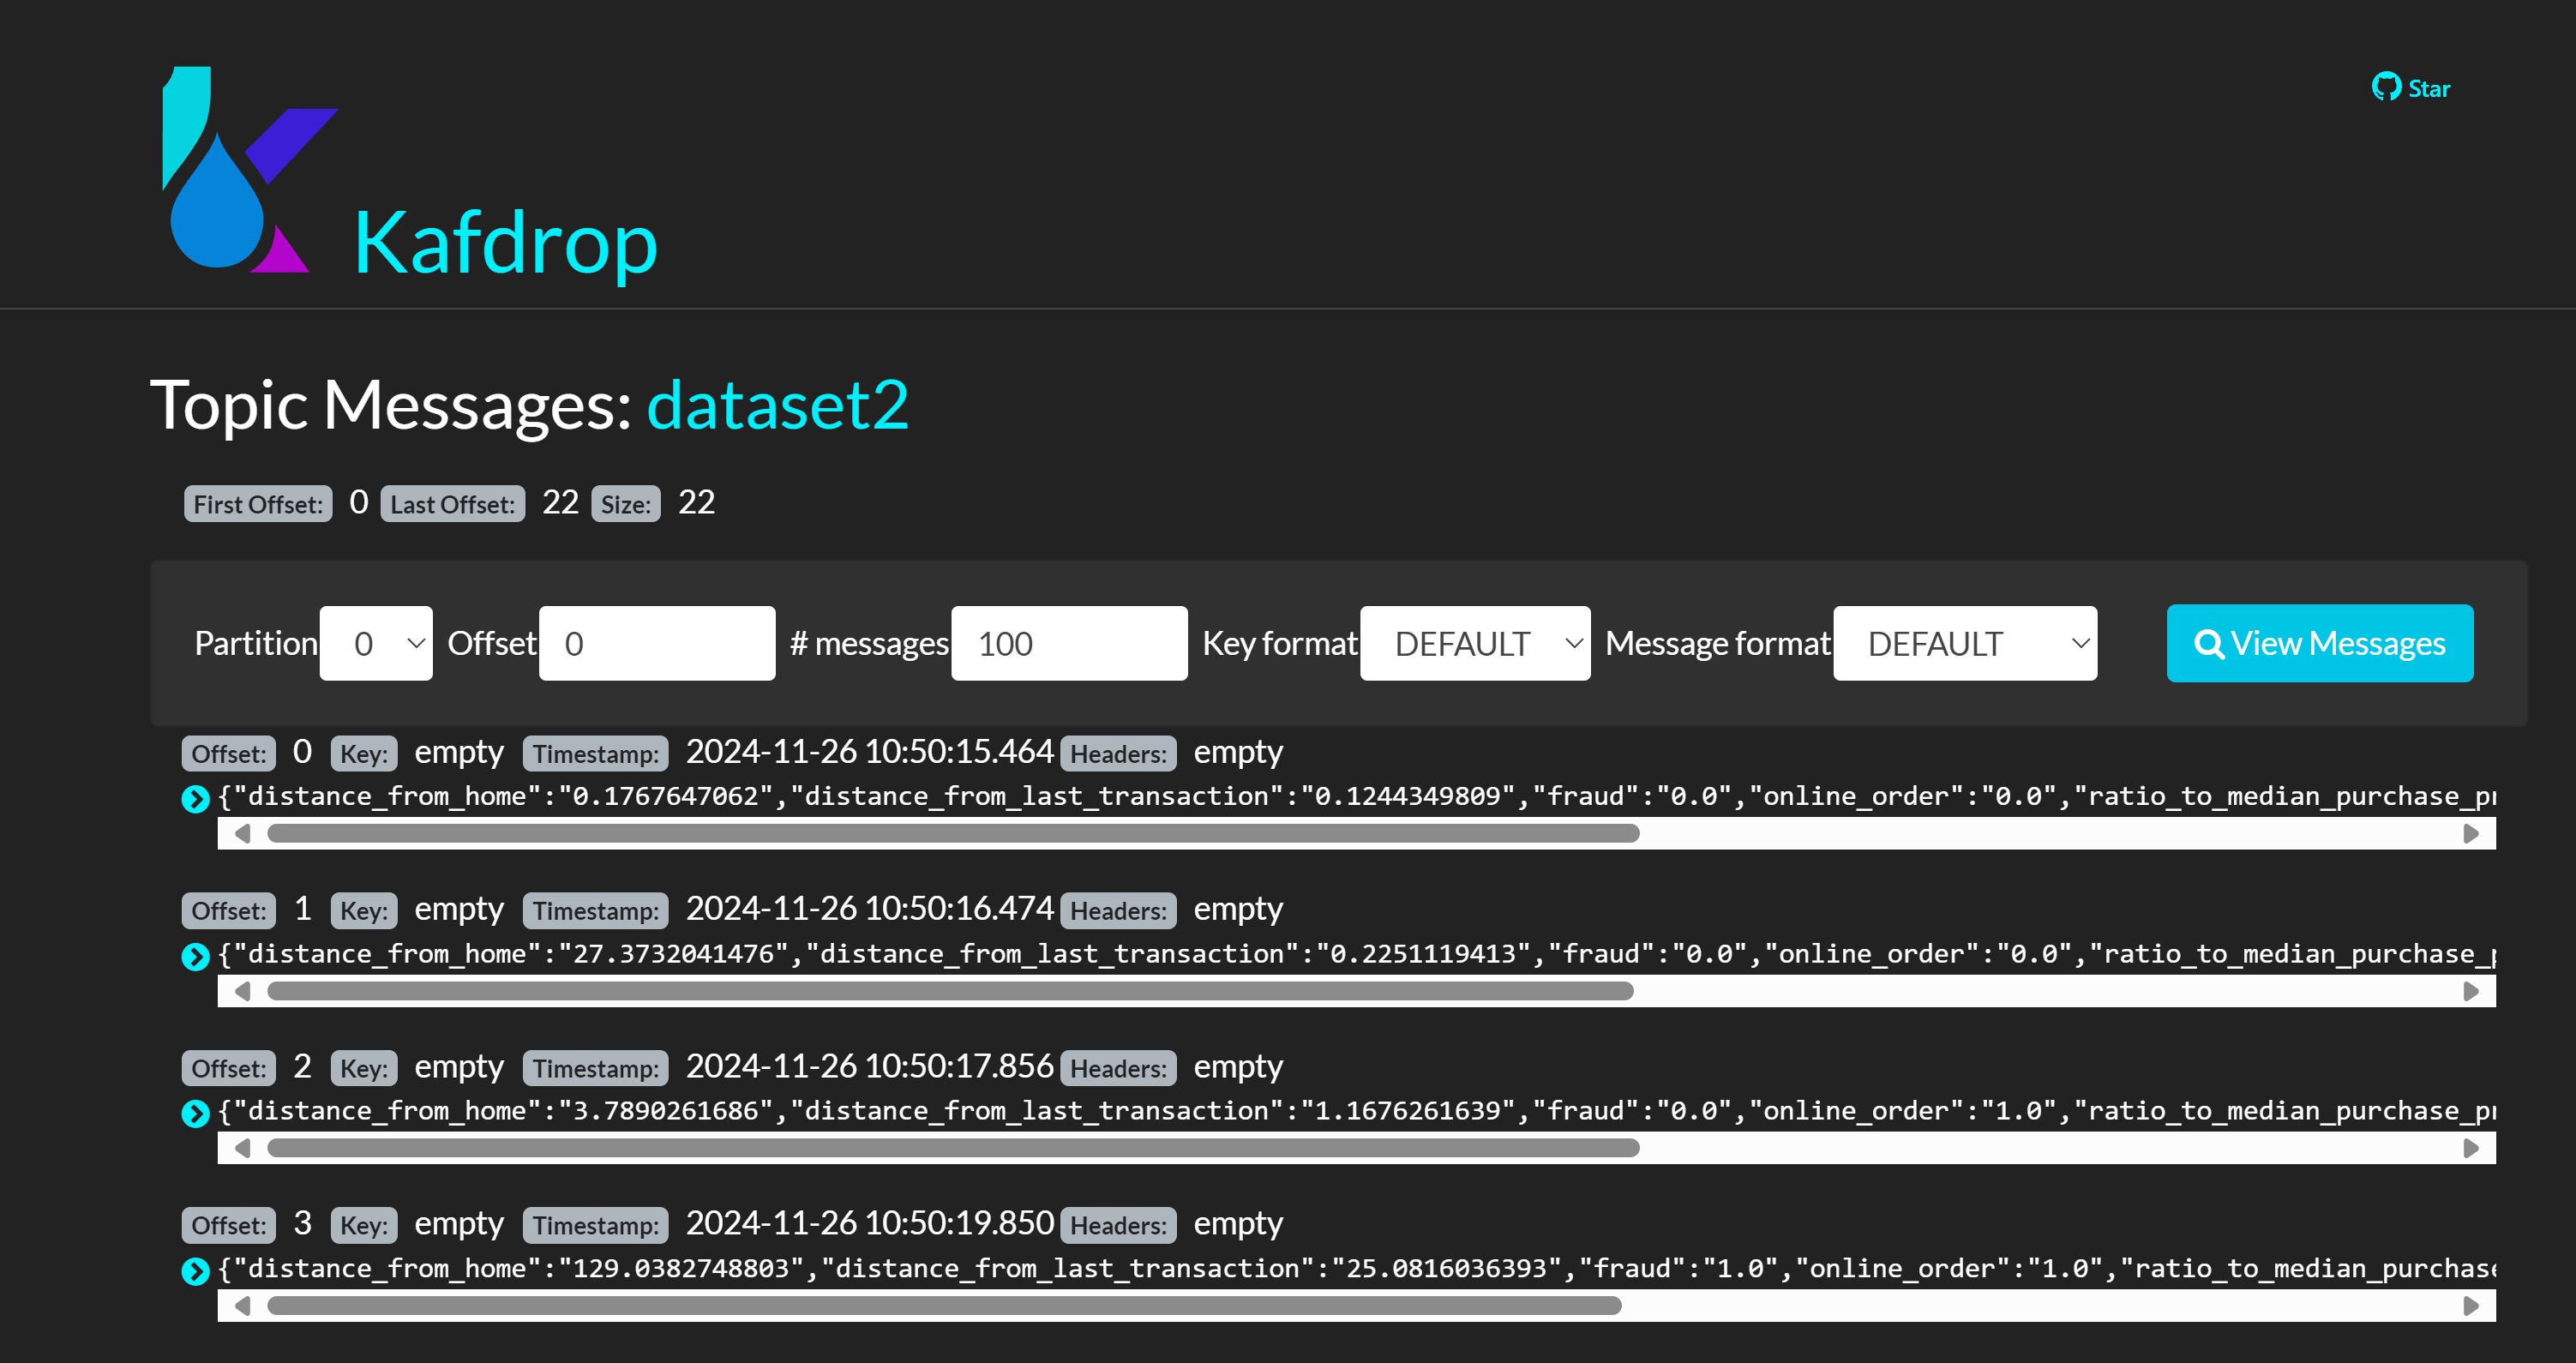
\includegraphics[width=0.95\textwidth]{images/m2-kafka-2.png}
  \caption{Kafka Dataset2}
  \label{fig:kafka2}
\end{figure}

\begin{figure}[h!]
  \centering
  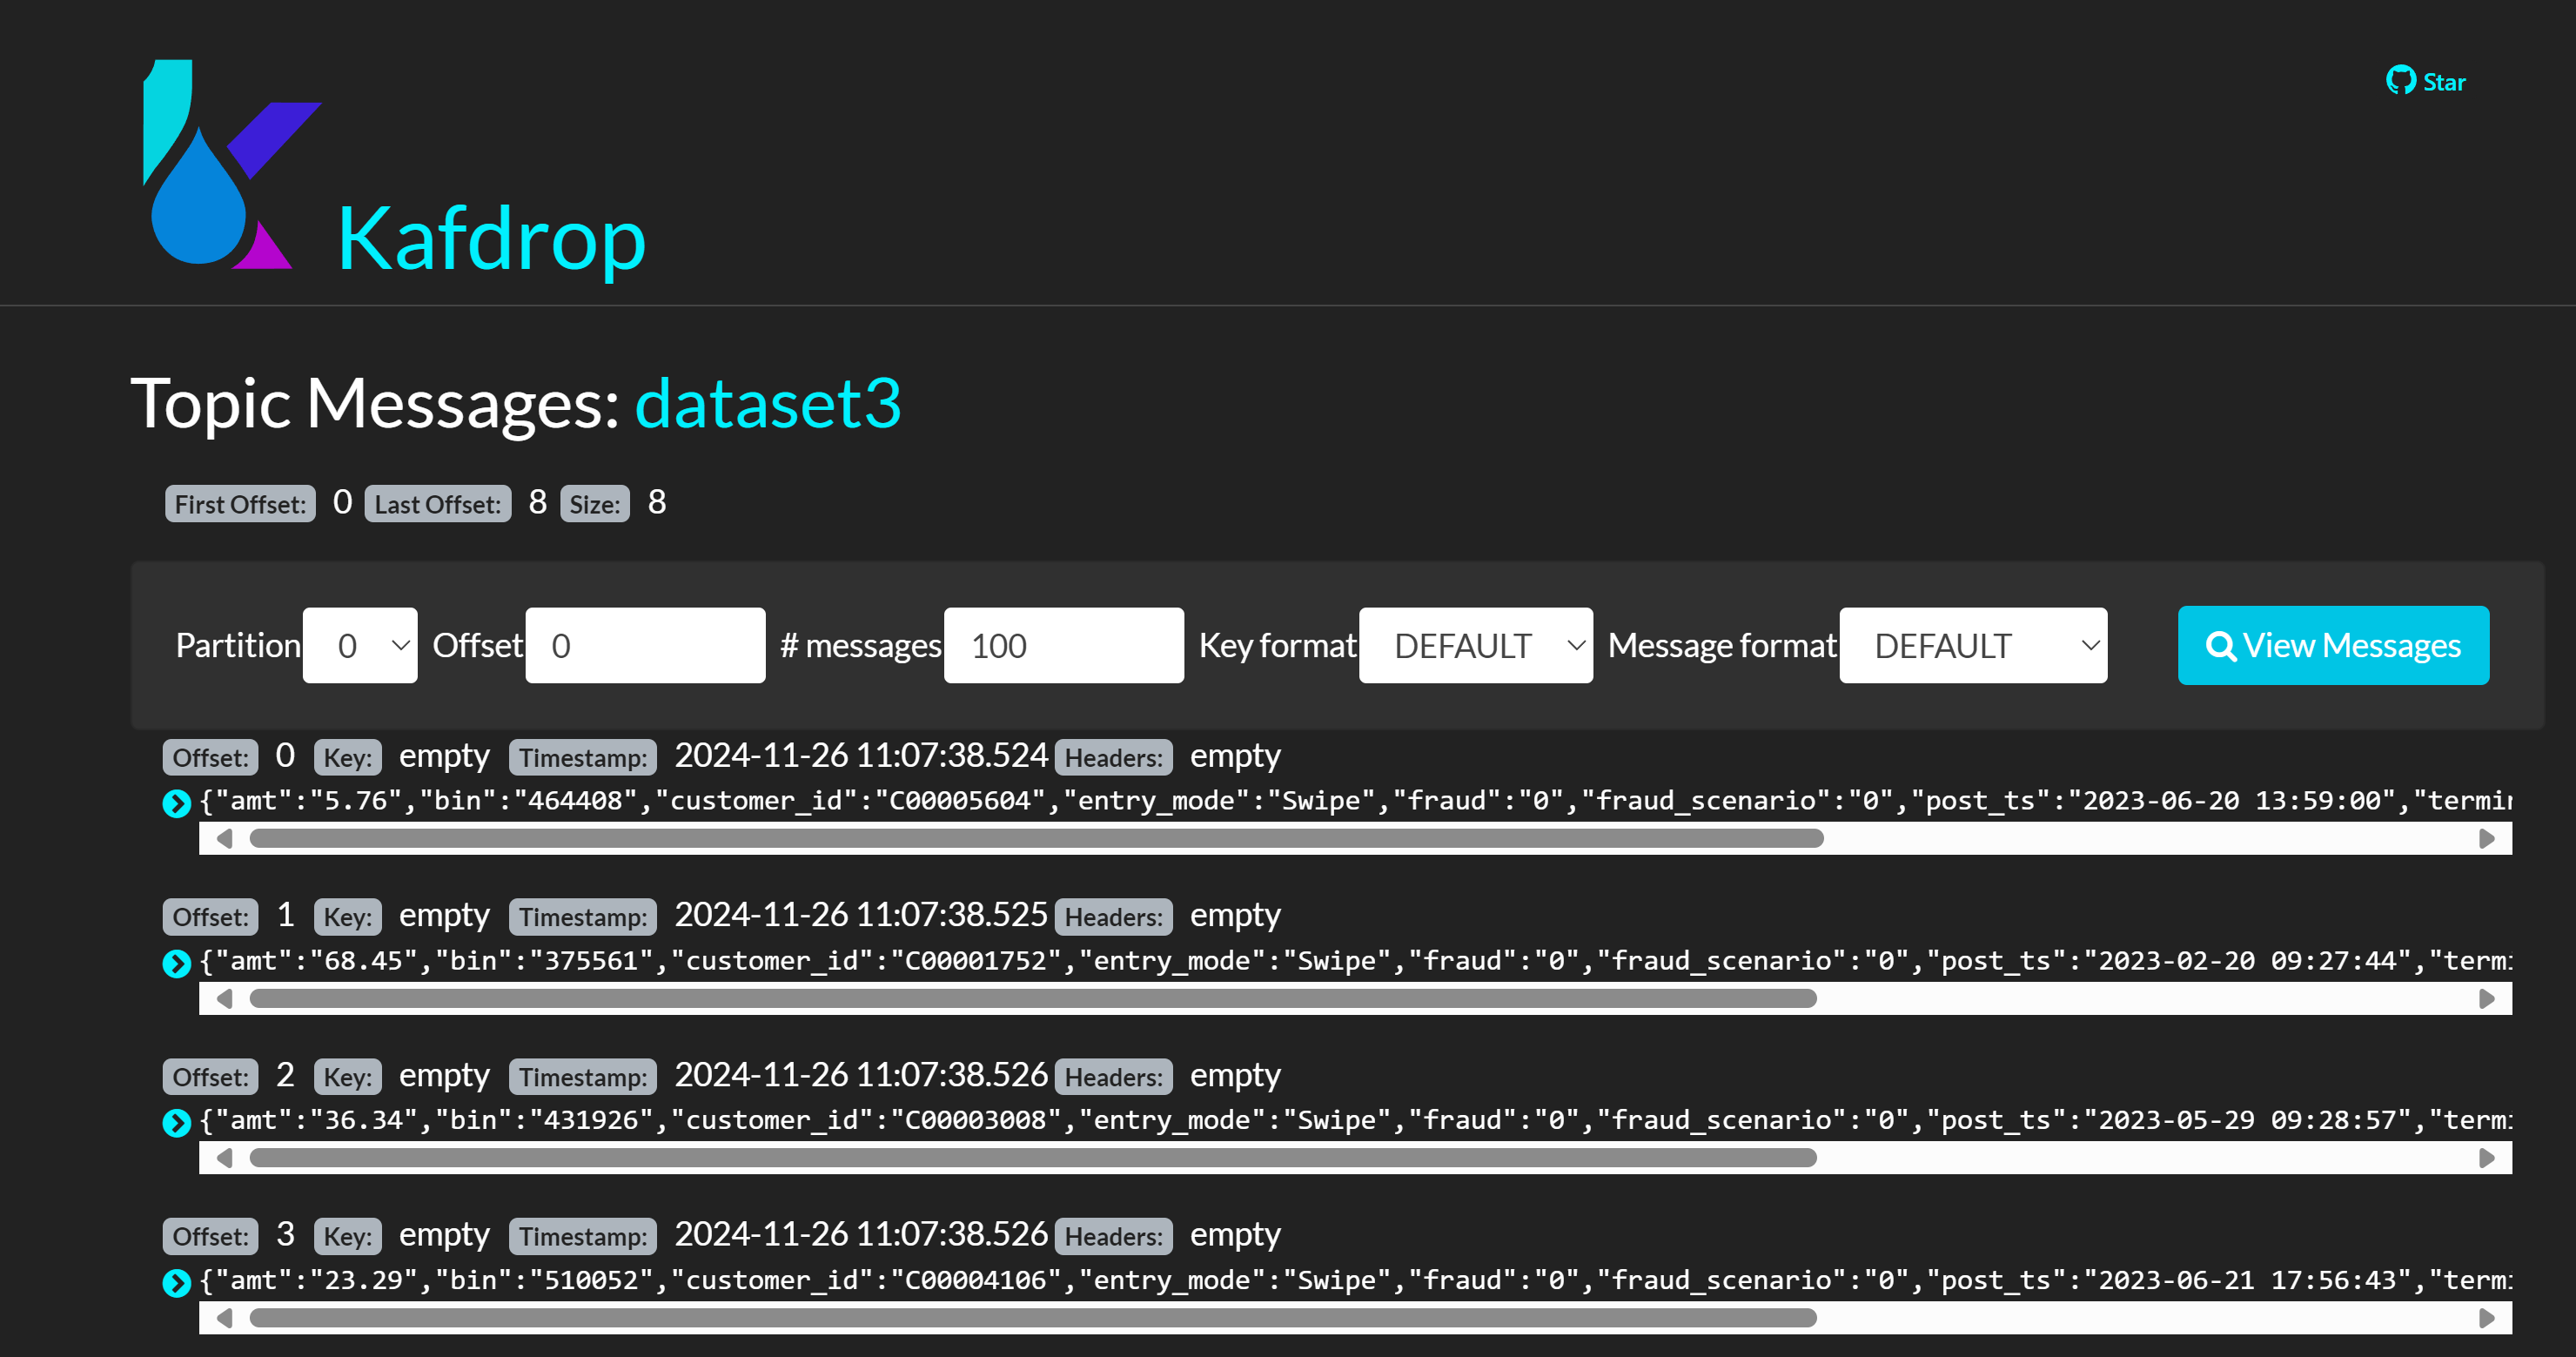
\includegraphics[width=0.95\textwidth]{images/m2-kafka-3.png}
  \caption{Kafka Dataset3}
  \label{fig:kafka3}
\end{figure}


\begin{figure}[h!]
  \centering
  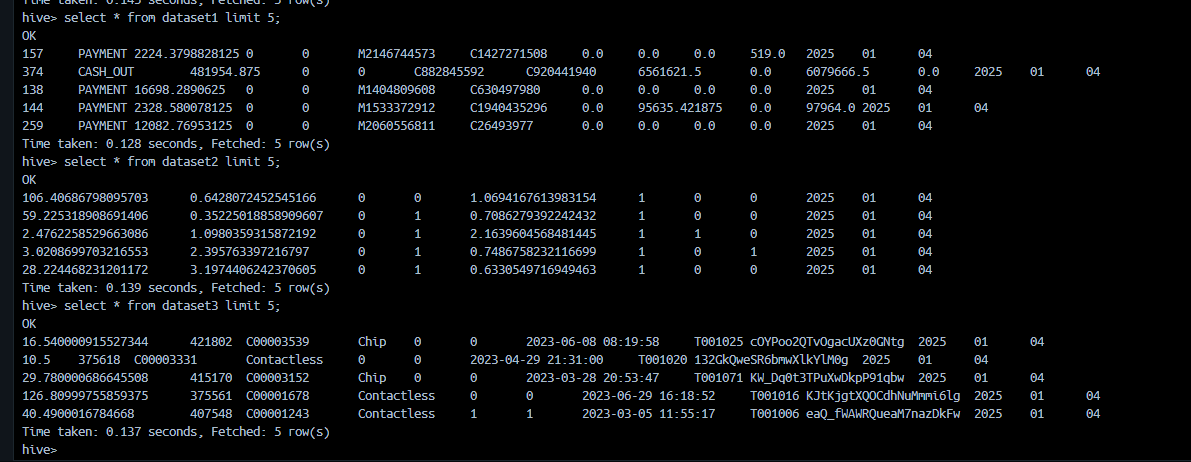
\includegraphics[width=0.95\textwidth]{images/m3-hive-tables.png}
  \caption{Hive data}
  \label{fig:hive1}
\end{figure}



\begin{figure}[h!]
  \centering
  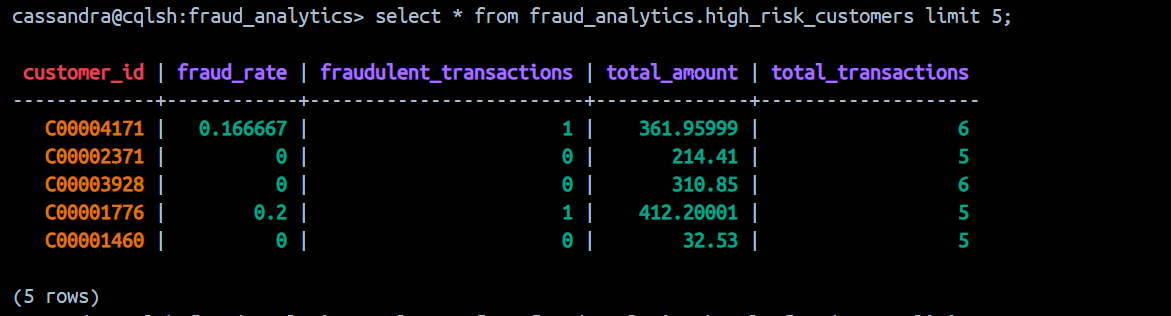
\includegraphics[width=0.95\textwidth]{images/m3-cassandra-batch-1.png}
  \caption{Cassandra batch processing views}
  \label{fig:cassandra-batch-1}
\end{figure}

\begin{figure}[h!]
  \centering
  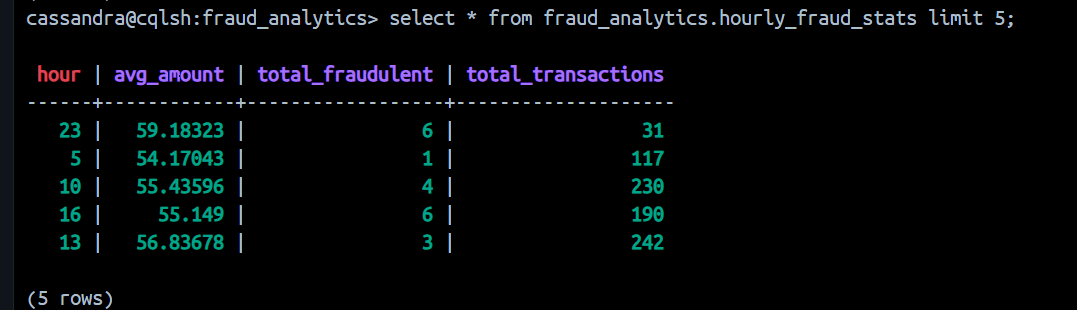
\includegraphics[width=0.95\textwidth]{images/m3-cassandra-batch-2.png}
  \caption{Cassandra batch processing views}
  \label{fig:cassandra-batch-2}
\end{figure}

\begin{figure}[h!]
  \centering
  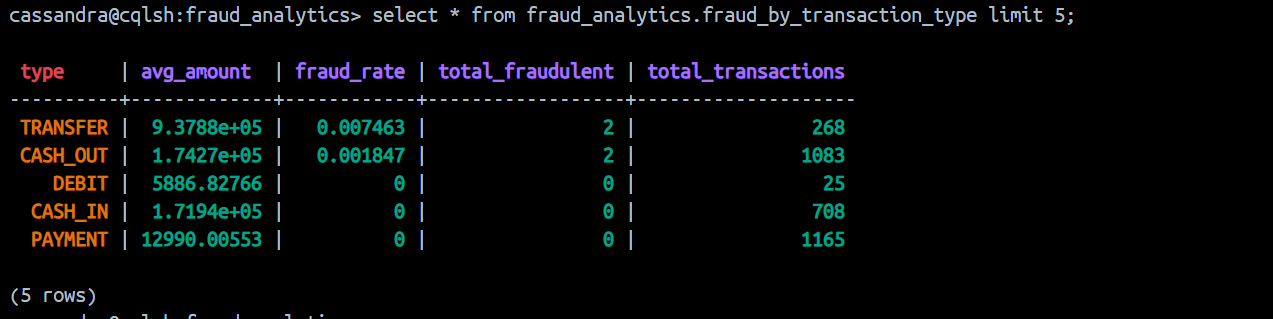
\includegraphics[width=0.95\textwidth]{images/m3-cassandra-batch-3.png}
  \caption{Cassandra batch processing views}
  \label{fig:cassandra-batch-3}
\end{figure}

\begin{figure}[h!]
  \centering
  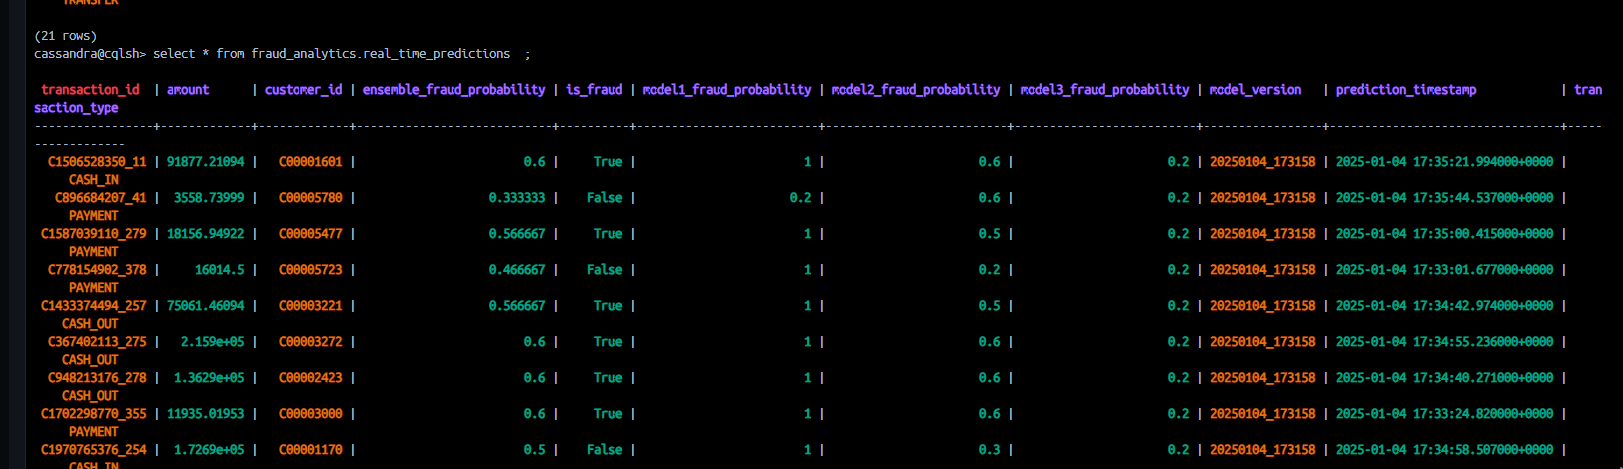
\includegraphics[width=0.95\textwidth]{images/m3-cassandra-streaming-processing.png}
  \caption{Cassandra stream processing views}
  \label{fig:cassandra-strean}
\end{figure}




\begin{figure}[h!]
  \centering
  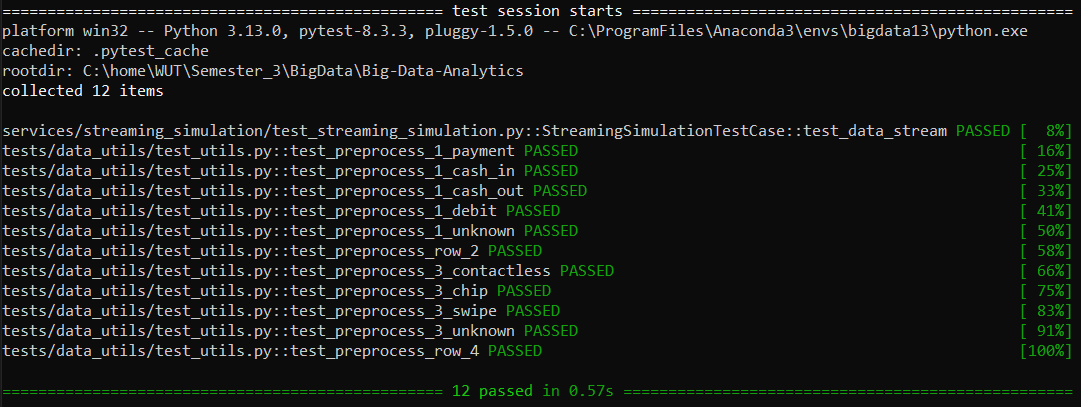
\includegraphics[width=0.95\textwidth]{images/unittests-M2.png}
  \caption{Unit testing result}
  \label{fig:unittests}
\end{figure}



\begin{figure}[h!]
  \centering
  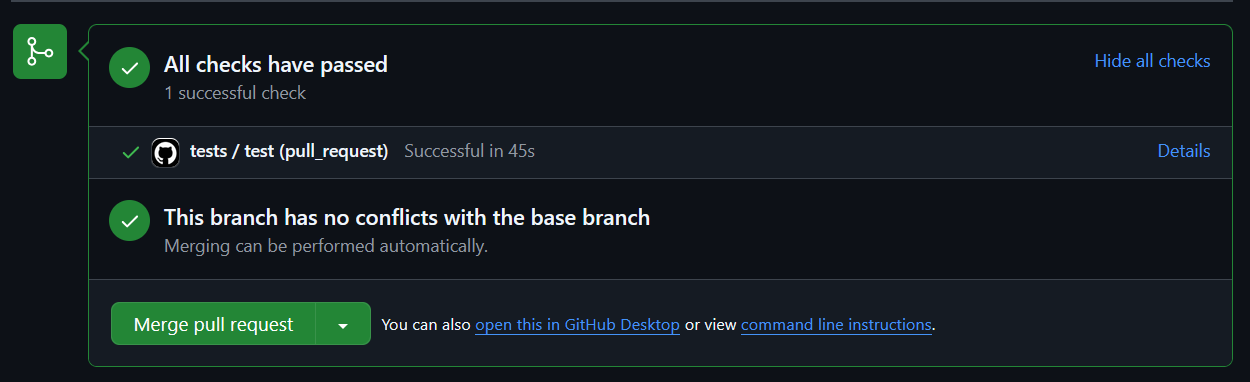
\includegraphics[width=0.95\textwidth]{images/github-checks-M2.PNG}
  \caption{GitHub checks before merge}
  \label{fig:github}
\end{figure}

\end{document}